\documentclass{article}

\usepackage[top=3cm, bottom=3cm, left=3cm, right=3cm]{geometry}

\usepackage[french]{babel}
\usepackage[utf8]{inputenc}
\usepackage[T1]{fontenc}

\usepackage[a4paper,colorlinks,linkcolor=darkgray,citecolor=red,urlcolor=blue]{hyperref}
\usepackage{pdfpages}
\usepackage{graphicx}
\usepackage{caption}
\usepackage{amsthm}
\usepackage{listings}

\newtheorem{ex}{Exemple}

\title{Rapport final : TriComp}

\author{}

\date{Vendredi 19 Décembre 2014}

\begin{document}

\makeatletter % Pour utiliser le "at" comme une commande interne.
  \begin{titlepage}
    \begin{center}
       {\LARGE \@title} \\
       \vspace{2cm}
       {\large \@date}
       \vspace{3cm}
    \end{center}
       {\large
       {William \textsc{Aufort} \hfill Julien \textsc{Bensmail} \\}
    \vspace{1cm}
       {\hfill coordinateur \\}
       {Agathe \textsc{Herrou}  \hfill Romain \textsc{Labolle} \\}
       \vspace{1cm}
       {chef de projet \\}
       \vspace{1.5cm}
       {Frédéric \textsc{Lang} \hfill Maxime \textsc{Lesourd} \\}
       {Laureline \textsc{Pinault} \hfill Léo \textsc{Stéfanesco} \\}}
       \vspace{2.5cm}
    \begin{abstract}
	Ce document présente le rapport final de notre projet TriComp. 
	% TODO : résumer le contenu du document
    \end{abstract}
  \end{titlepage}
\makeatother

\newpage

\tableofcontents

\newpage

\section*{Introduction}

Le tricot est un art que l'on imagine souvent réservé aux personnes âgées.

Les magazines de tricot présententent souvent des modèles à réaliser soi-même, combinant différents points. Il est cependant vite fastidieux d'écrire la suite des 
instructions à suivre pour réaliser une pièce. Notre but ici était donc de réaliser un logiciel permettant d'une part de décrire des pièces de tricot de manière \emph{user-friendly}, et, à partir de cette description, de générer une suite d'instructions à destination du tricoteur permettant de réaliser la pièce en question. 

Cette opération de traduction d'un langage de ``haut niveau'' (l'ensemble des pièces du tricot) vers un langage de ``bas niveau'' (les instructions) rappelait fortement le principe d'un compilateur, c'est pourquoi 
nous avons d'abord considéré notre projet comme un ``compilateur de tricot''. À l'instar de la compilation d'un langage de programmation informatique, cette 
compilation de tricot était susceptible de mener à des problèmes théoriques intéressants, à mesure que l'on enrichirait le langage.
% ici, on explique nos motivations, la genèse du projet
% motivations : le tricot c'est bien, mais vite fastidieux de construire des modèles à la main
% Magazines de tricot : proposent souvent des modèles combinant de nombreux points différents, mais fastidieux de construire le modèle et de calculer où il faut faire quelle opération (tricoter une maille à l'endroit ou à l'envers, croiser des mailles, en ajouter, en enlever...)
% autre motivation : intérêt théorique, potentiels problèmes mathématiques intéressants peuvent surgir (en pratique on n'est pas allés assez loin pour les rencontrer)

\subsection*{Lexique du tricot} % ou : Quelques mots sur le tricot

% définition d'un certain nombre de mots : maille, point, ouvrage ; et description rudimentaire des techniques

Le vocabulaire du tricot peut sembler un peu obscur aux non-initiés, voici donc quelques définitions :

\begin{itemize}
% + rang
\item une \emph{maille} est l'unité de base d'un tricot. Il s'agit de la boucle qui constitue l'étoffe en étant reliée à ses voisines, horizontalement car 
  partageant la même portion de fil, verticalement car ces boucles sont imbriquées les unes dans les autres. Elle peut être à l'endroit ou à l'envers, selon la 
  manière dont la boucle est réalisée.
\item un \emph{point} est une manière de combiner les différentes opérations réalisables sur les mailles (les tricoter à l'endroit, à l'envers, en tricoter 
  plusieurs ensemble, croiser plusieurs mailles \dots)
\item l'\emph{ouvrage} désigne la pièce de tricot tout entière, par exemple l'écharpe ou le pull.
\item une \emph{diminution} est la suppression d'une maille dans le cours de l'ouvrage ; une technique courante consiste à tricoter ensemble 
  deux mailles. Symétriquement, une \emph{augmentation} est une maille ajoutée dans le cours de l'ouvrage ; une technique 
  courante consiste à enrouler le fil sur l'aiguille pour former une nouvelle maille (on parle alors de \emph{jeté}).
\end{itemize}

Le tricot est réalisé à l'aide d'aiguilles, qui servent d'une part à maintenir les boucles libres (pour éviter qu'elles ne se défassent et libèrent les boucles du 
rang précédent qu'elles retiennent), d'autre part à former de nouvelles boucles.

\newpage

\section{Travail réalisé}

Le travail que nous prévoyions de réaliser impliquait d'une part de définir différents langages de ``programmation'' du tricot (un langage de haut niveau pour 
décrire de manière rigoureuse les ouvrages, et un langage de bas niveau correspondant aux mailles à tricoter), d'autre part d'écrire un compilateur réalisant la 
traduction d'un langage vers l'autre, et enfin de réaliser une interface graphique permettant de les manipuler intuitivement et de visualiser les pièces en cours de 
définition.
Nous détaillons dans cette partie le travail qui a été réalisé dans chacun de ces objectifs. Nous rappelons que tout le travail (logiciel, documents et site web) sont disponibles et consultables sur le dépôt Git du projet TriComp. (\url{https://github.com/TriComp/}).

\subsection{Définition des langages}

Nous avons été amenés au cours de ce projet à définir deux langages, l'un purement statique, puisque servant à décrire les ouvrages de tricot, l'autre dyamique, car 
décrivant le processus de réalisation du tricot.

\subsubsection{Langage descriptif}

Une première version du langage descriptif avait été détaillée dans le rapport mi-parcours. Quelques modifications ont été effectuées depuis. Nous exposerons donc ici le langage final, les modifications effectuées ainsi que leur intêret, le tout illustré par un exemple. \\

L'idée générale est de concevoir une langage capable décrire un tricot de la façon la plus globale possible. Dans les (rares) logiciels de tricot qui existent, le tricot est décomposé en sa plus petite entité : la maille (cf figure \ref{logiciel}). L'avantage de cette décomposition atomique est que l'on peut réaliser des choix de points avec une très bonne précision. Notre démarche, quand à elle, propose une vision du tricot plus globale, et donc beaucoup plus simple.

\begin{figure}[!ht]
  \centering
  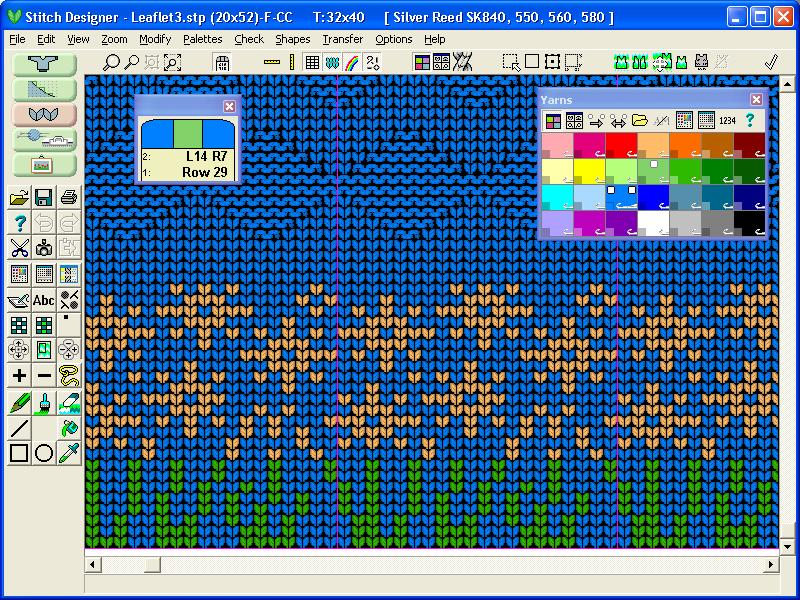
\includegraphics[scale=0.3]{../img/grid.jpg}
  \caption{Le logiciel Stitch Designer propose une vue très précise du tricot, mais celui-ci a donc une taille beaucoup trop importante (comme en témoignent les barres de défilement à droite et en bas de la fenêtre}
  \label{logiciel}
\end{figure}




\subsubsection{Langage de bas niveau}

\subsection{Compilateur}

\subsubsection{Langage descriptif vers langage bas niveau}

\subsubsection{Langage bas niveau vers langage naturel}




\subsection{Interface graphique}

% inclure des captures d'écran etc

% le midterm report met ici le site web, mais je ne suis pas si sûre que ça soit très pertinent
% -> autre section ? ("Communication")



\section{Améliorations possibles}

% ici, on parlera des autres versions du langage, des améliorations qu'on aurait pu apporter à l'interface graphique...
Le manque de temps et de moyens humains nous a empêché de mettre en place la totalité des fonctionnalités que nous avions prévues, notamment en ce qui concerne les 
types de points gérés par le langage (la version actuelle ne gère que les points à base de mailles à l'endroit et à l'envers).

\subsection{Langage de description}
% à réécrire pour le rendre sexy et vendeur
En ayant plus de temps à notre disposition, nous pourrions intégrer au langage d'une part les diminutions et augmentations, d'autre part les tresses. Ces 
différentes 

\subsection{Interface graphique}




\section{Résultats théoriques}

\subsection{Algorithmes de répartition des diminutions}

\subsection{Allocation d'aiguilles}





\end{document}
